\section{Candidate Assessment and Request Selection}
Figure~\ref{fig:candidate_decision_full} distinguishes a candidate action from the request outcome. The input is an incoming task, the stored question and answer, and the retrieval similarity. Structural checks can reject a changed number, polarity, named work, or unsupported answer type before model inference. Configured technical and applicability guards can also act on recognized actions, environments, and versions. These guards are optional; the experimental task-specific classifier is not a normal deployed verifier. Unresolved candidates go to the pinned answer-assertion NLI model. An unavailable model, overlong pair, uncertainty interval, or exhausted time budget produces VERIFY, an abstention rather than a judgement that the answer is false.

The cache coordinator assesses up to a configured limit and aggregates the resulting ACCEPT, VERIFY, and REJECT actions. A first ACCEPT does not guarantee a request HIT: accepted answers may conflict, a plausible lower-ranked candidate may remain unassessed, or the verification budget may expire. Only a selected answer whose Redis hash still matches the candidate may be served. The gateway also rechecks the principal before returning it. These checks trade some valid reuse for explicit uncertainty boundaries, as the measured valid misses in Chapter~6 show.

\clearpage\thispagestyle{plain}
\begin{figure}[H]\centering
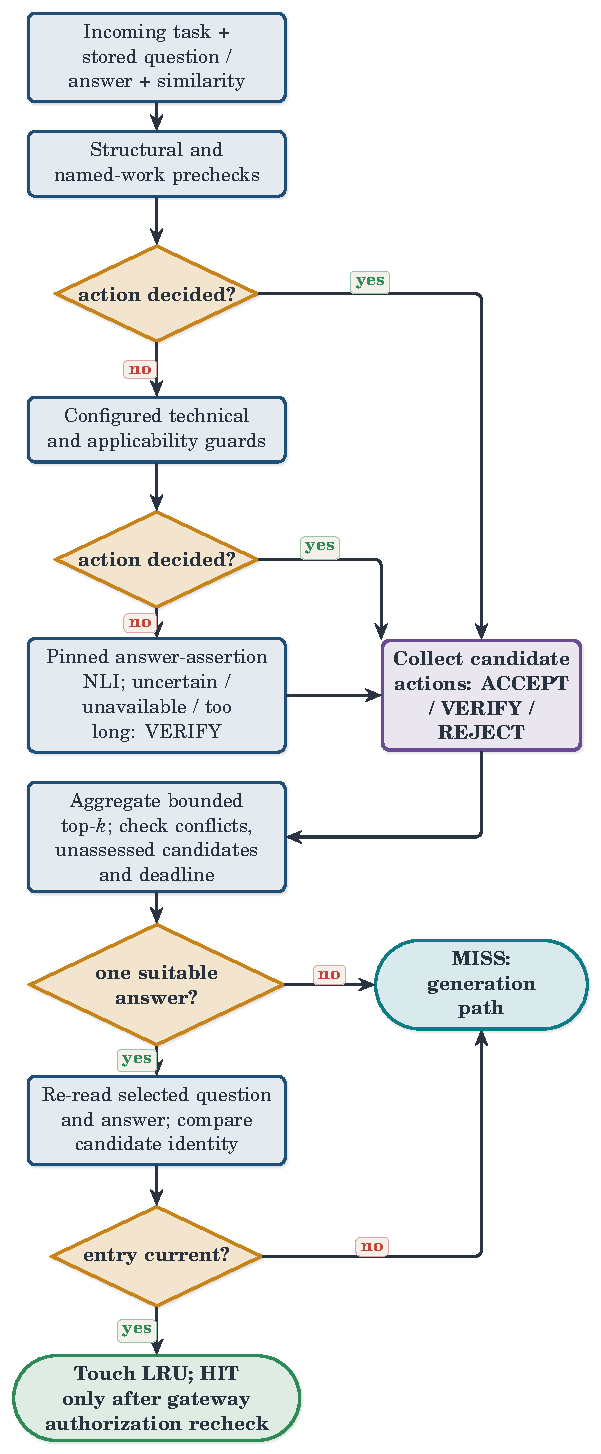
\includegraphics[width=\textwidth,height=.79\textheight,keepaspectratio]{candidate_decision.pdf}
\caption{Candidate action precedes top-$k$ selection and final request outcome.}\label{fig:candidate_decision_full}
\end{figure}
\clearpage

\section{Semantic Hit Interaction}
Figure~\ref{fig:hit_sequence_full} is specifically the semantic HIT path after an exact-key miss. The gateway has already authenticated the caller and resolved the authorized scope. The cache coordinator reads the scope-local exact key, receives no current entry, asks the local embedder for a normalized vector, and requests a tenant-filtered shortlist from RedisSearch. The bounded-candidate annotation refers to Figure~\ref{fig:candidate_decision_full}: each eligible candidate can receive a precheck or verifier action, and the coordinator then checks conflicts and remaining plausible candidates.

For a selected candidate the coordinator re-reads the Redis hash and compares its stored question and answer. If the record has expired or changed, the request becomes a MISS. Otherwise a served semantic HIT updates LRU recency only; it does not renew the entry TTL. At this checkpoint the semantic identity read precedes the recency update; the operation is not an atomic read-and-serve transaction, so a subsequent mutation window remains. The cache coordinator returns the answer and trace to the gateway, which rechecks authorization and sends the client the HIT response. The provider has no role on this branch. The exact shortcut is described separately because it can return without embedding or NLI and touches recency before a confirming re-read in the current implementation.

\clearpage
\thispagestyle{plain}
\begin{figure}[H]\centering
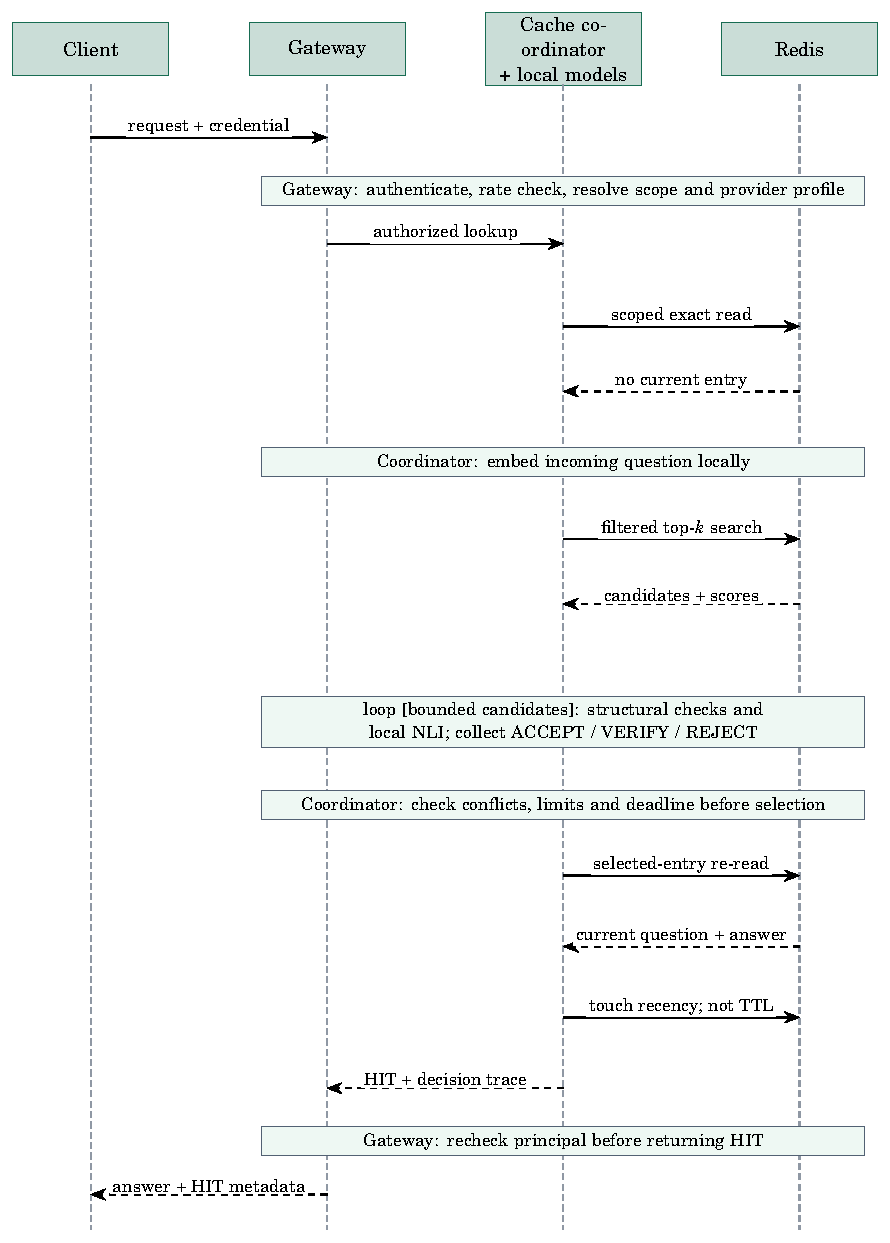
\includegraphics[width=\textwidth,height=.79\textheight,keepaspectratio]{hit_sequence.pdf}
\caption{Semantic HIT sequence after an exact-key miss.}\label{fig:hit_sequence_full}
\end{figure}
\clearpage

\section{JSON Miss and Fallback Interaction}
Figure~\ref{fig:fallback_sequence_full} follows a JSON MISS or BYPASS. The cache coordinator returns a reason: an empty scope, no suitable candidate, a verifier abstention, a conflict, or a stale selected entry. The gateway checks the principal again and charges an admitted miss before provider work. A rejected or unavailable admission result exits without generation. A JSON MISS can join process-local singleflight; a BYPASS calls the generator directly. A same-worker follower receives the leader's answer without its own provider call or cache write. Streaming does not use this JSON coalescing path.

The provider registry selects an intended configured route and prefetches the first provider event before it returns the selected provider name and a wrapped event stream. The gateway then iterates that stream to receive the remaining events. The JSON generator accumulates content and requires one normal terminal completion and a nonempty bounded answer. Timeout, provider error, or incomplete completion leads to an explicit error with no storage. A completed answer is classified against the request scope and provider route. A no-store answer, BYPASS, or successful alternate provider route skips storage under the intended cache identity. Eligible responses may be written to a shared workspace or downgraded to private scope. Storage success, refusal, timeout, and failure remain separate metadata outcomes; a failed write does not discard a completed provider answer. The guarded annotations identify these alternatives. Worker-local components are grouped into participant lanes to keep the portrait diagram readable; the text separates their responsibilities.

\clearpage
\thispagestyle{plain}
\begin{figure}[H]\centering
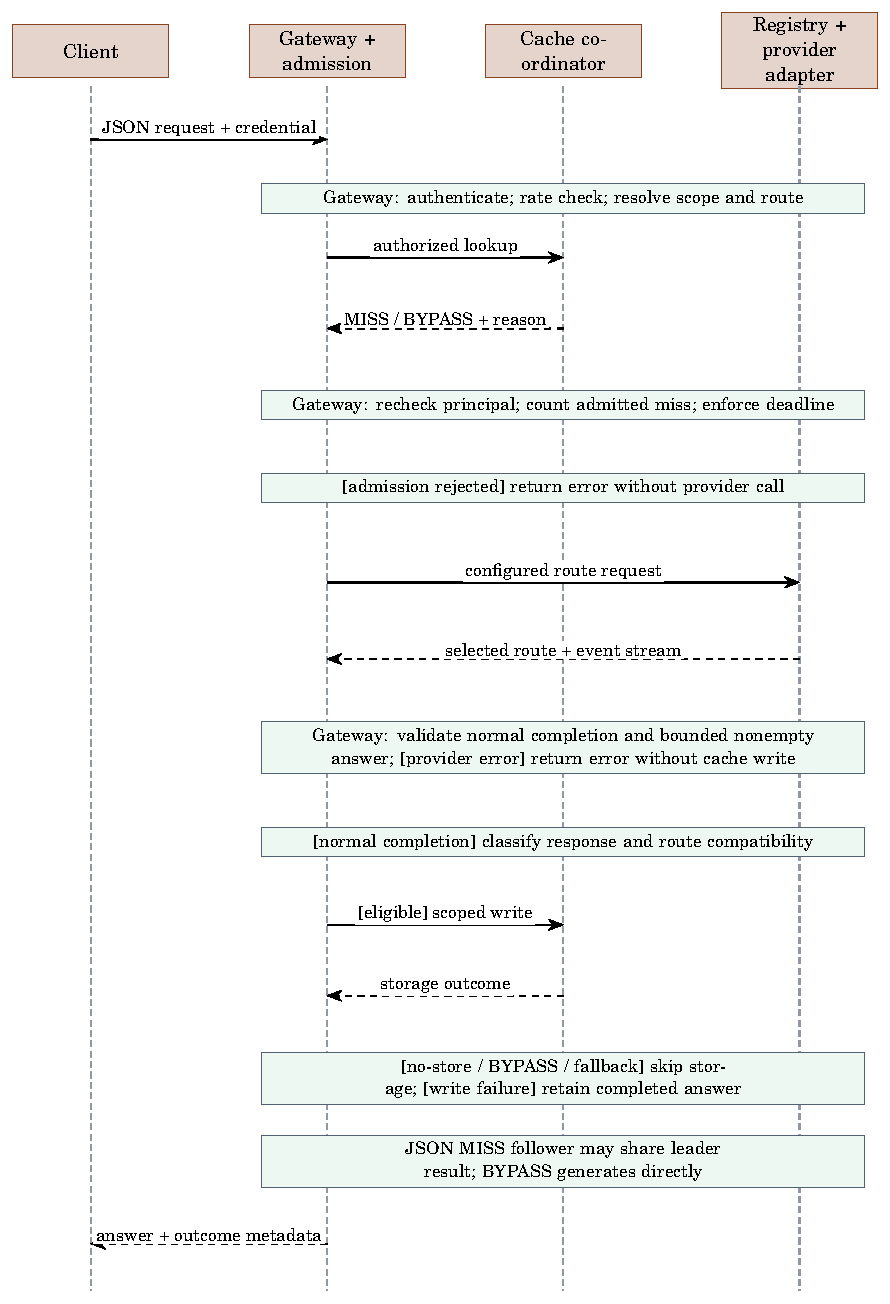
\includegraphics[width=\textwidth,height=.79\textheight,keepaspectratio]{fallback_sequence.pdf}
\caption{JSON MISS/BYPASS sequence with admission and storage alternatives.}\label{fig:fallback_sequence_full}
\end{figure}
\clearpage

\clearpage\thispagestyle{plain}
\section{Organization, Workspace, and Private Identity}
Figure~\ref{fig:org_scope_full} keeps Alice and Carol inside Organization A and Bob inside Organization B. Alice can write an eligible completed answer to a shared workspace and Carol can read it only with matching membership and \texttt{cache:shared} permission. Alice's private subject/application scope has no read path from Carol. Bob's similarly worded request resolves to Organization B's separate opaque identity; the denied cross-organization attempt is an authorization boundary rather than a low similarity score. The diagram is conceptual and does not expose raw credentials or Redis key material.

Automatic scope resolution comes from server-side directory membership, defaults, content eligibility, and provider profile. An explicit API request for a scope cannot grant missing permission. Provider-profile compatibility is a second constraint: even two authorized members need the same compatible route identity for reuse. A response containing private context can be narrowed to Alice's private scope despite an originally eligible workspace request. Such classification is heuristic, so it is not a complete privacy guarantee.

\begin{figure}[H]\centering
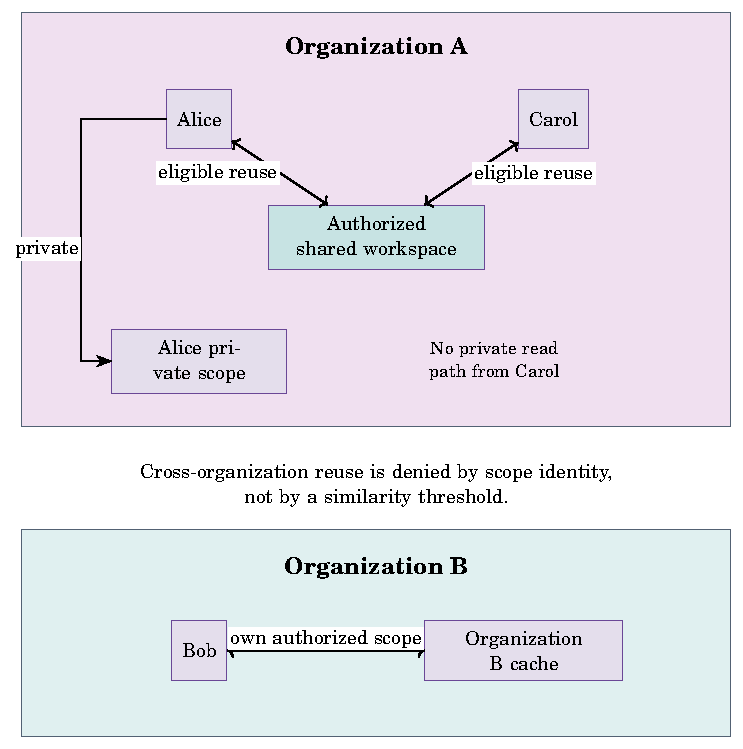
\includegraphics[width=\textwidth,height=11cm,keepaspectratio]{organization_scope.pdf}
\caption{Authorized workspace sharing and organization/private isolation.}\label{fig:org_scope_full}
\end{figure}
\clearpage

\clearpage\thispagestyle{plain}
\section{Logical Redis Storage and Index}
Figure~\ref{fig:storage_full} is a logical model, not a relational schema. A versioned namespace encodes policy, model, and provider compatibility. Within it, an opaque authorized scope tag and a digest of the stored question identify an entry hash. The hash contains question and answer text, the tenant tag, optional response-scope metadata, and, for RedisSearch semantic mode, a binary FLOAT32 embedding vector. The HNSW index uses the tenant TAG filter and COSINE distance to shortlist nearby entries. Approximate search can miss a suitable candidate; it does not assess the answer's applicability.

Redis membership sets and sorted sets record IDs, recency, sizes, organization expiry accounting, and quota totals. The entry hash has a finite TTL. A HIT touches LRU ordering, not TTL; expiry can occur without another lookup. Quota pressure can evict a young entry independently of its age. Redis itself needs a finite production memory setting. A process-local vector matrix is an alternative backend with different lookup and synchronization behavior, not an additional RedisSearch table. Redis never calls the LLM provider.

\begin{figure}[H]\centering
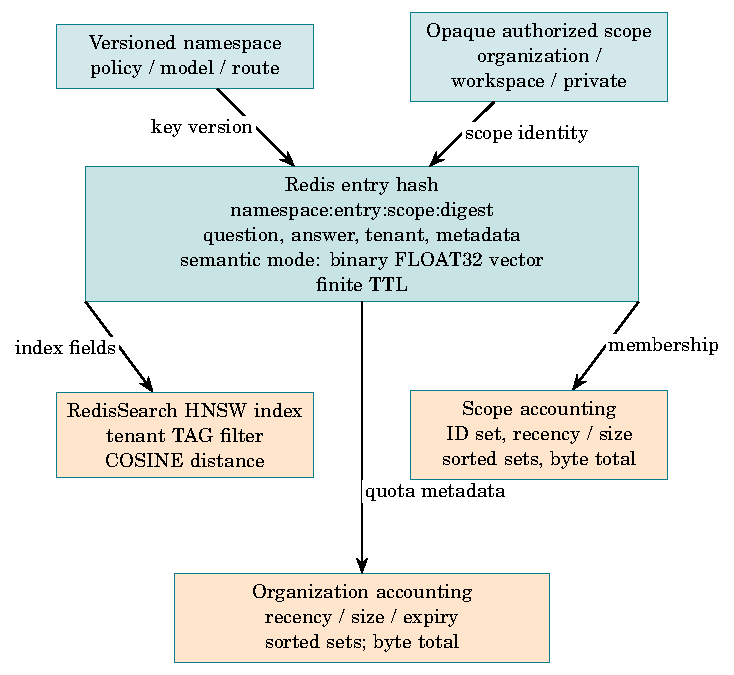
\includegraphics[width=\textwidth,height=.79\textheight,keepaspectratio]{storage_design.pdf}
\caption{Redis hash, vector index, and scope/organization accounting.}\label{fig:storage_full}
\end{figure}
\clearpage

\clearpage\thispagestyle{plain}
\section{Local Deployment and Process State}
Figure~\ref{fig:deployment_full} depicts the actual local Compose configuration and the separate external-provider variant. The gateway image contains FastAPI, adapters, and application policy artifacts. The local \texttt{MockProvider} executes inside the gateway process. An OpenAI-compatible or Gemini profile sends HTTP traffic to the configured external provider, independently of Redis protocol traffic. Redis Stack has a named \texttt{redis-data} volume mounted at \texttt{/data}; the base Compose file declares no gateway model or configuration mount. The organization-demo overlay illustrated here adds a read-only configuration mount and a persistent model-cache volume. Models can load into each worker's own memory, while Redis entries, index, admission and quota state are shared.

Locks, memoization, and JSON singleflight are process-local. A second worker can see Redis entries but can still make a duplicate provider call and adds its own model memory. A managed multiworker deployment is a future scale-out design, not a measured capability of this local diagram. The measured mock and controlled-provider runs do not establish external-provider cost or latency.

\begin{figure}[H]\centering
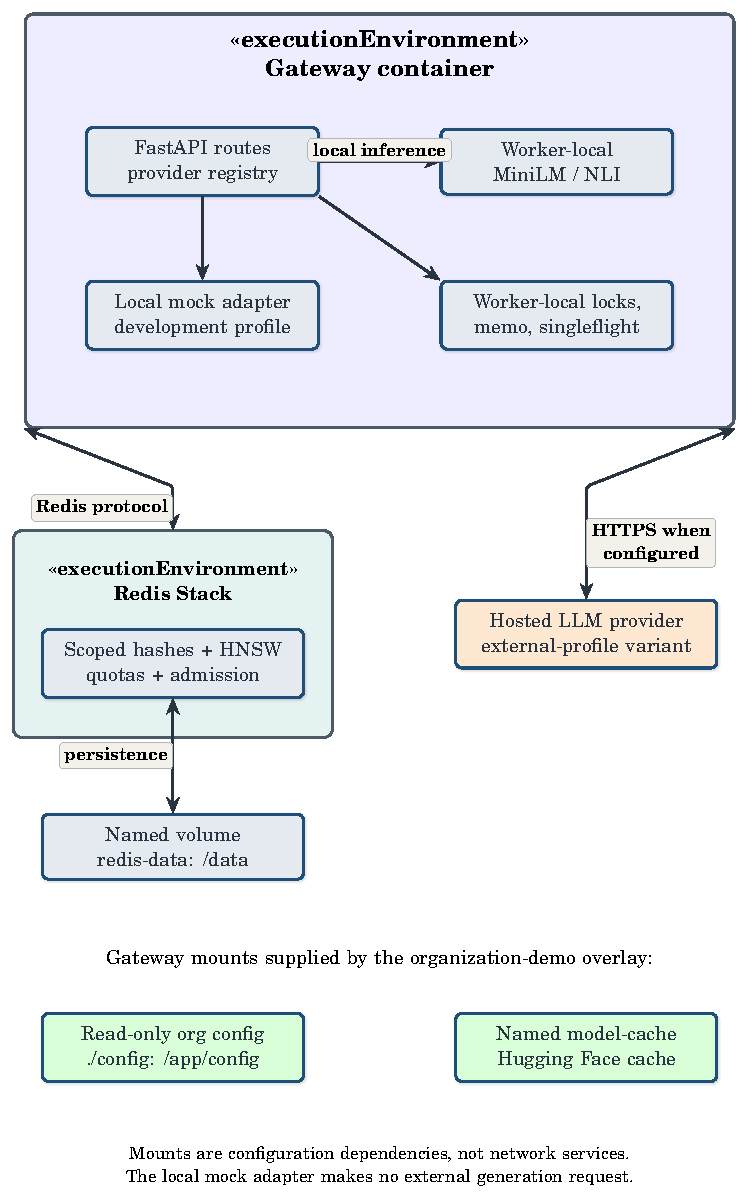
\includegraphics[width=\textwidth,height=.79\textheight,keepaspectratio]{deployment.pdf}
\caption{Compose containers, shared Redis state, and optional external HTTP.}\label{fig:deployment_full}
\end{figure}
\clearpage

\section{Startup, Readiness, and Cache Residence}
Figure~\ref{fig:startup_full} begins with configuration validation and a Redis connection. Startup loads the organization directory, constructs the cache, model wrapper, registries, rate limiter, and metrics. Semantic MiniLM mode warms an embedding; configured answer-policy prewarm loads the verifier. RedisSearch semantic mode probes the vector dimension and creates or validates the HNSW schema. A configuration, Redis, model, or schema failure can prevent readiness. In exact mode the semantic model and index branches are not required.

The actual probe routes have distinct boundaries: \texttt{/live} gives a minimal process response, while \texttt{/ready} and \texttt{/health} share the dependency check in \texttt{app/main.py}. The Dockerfile's \texttt{HEALTHCHECK} calls \texttt{/health}, so its status includes Redis and configured component checks rather than liveness alone. In production these probe responses expose only the status, while \texttt{/admin/config} is authenticated and returns details. The figure does not create a separate, nonexistent liveness API.

\begin{figure}[H]\centering
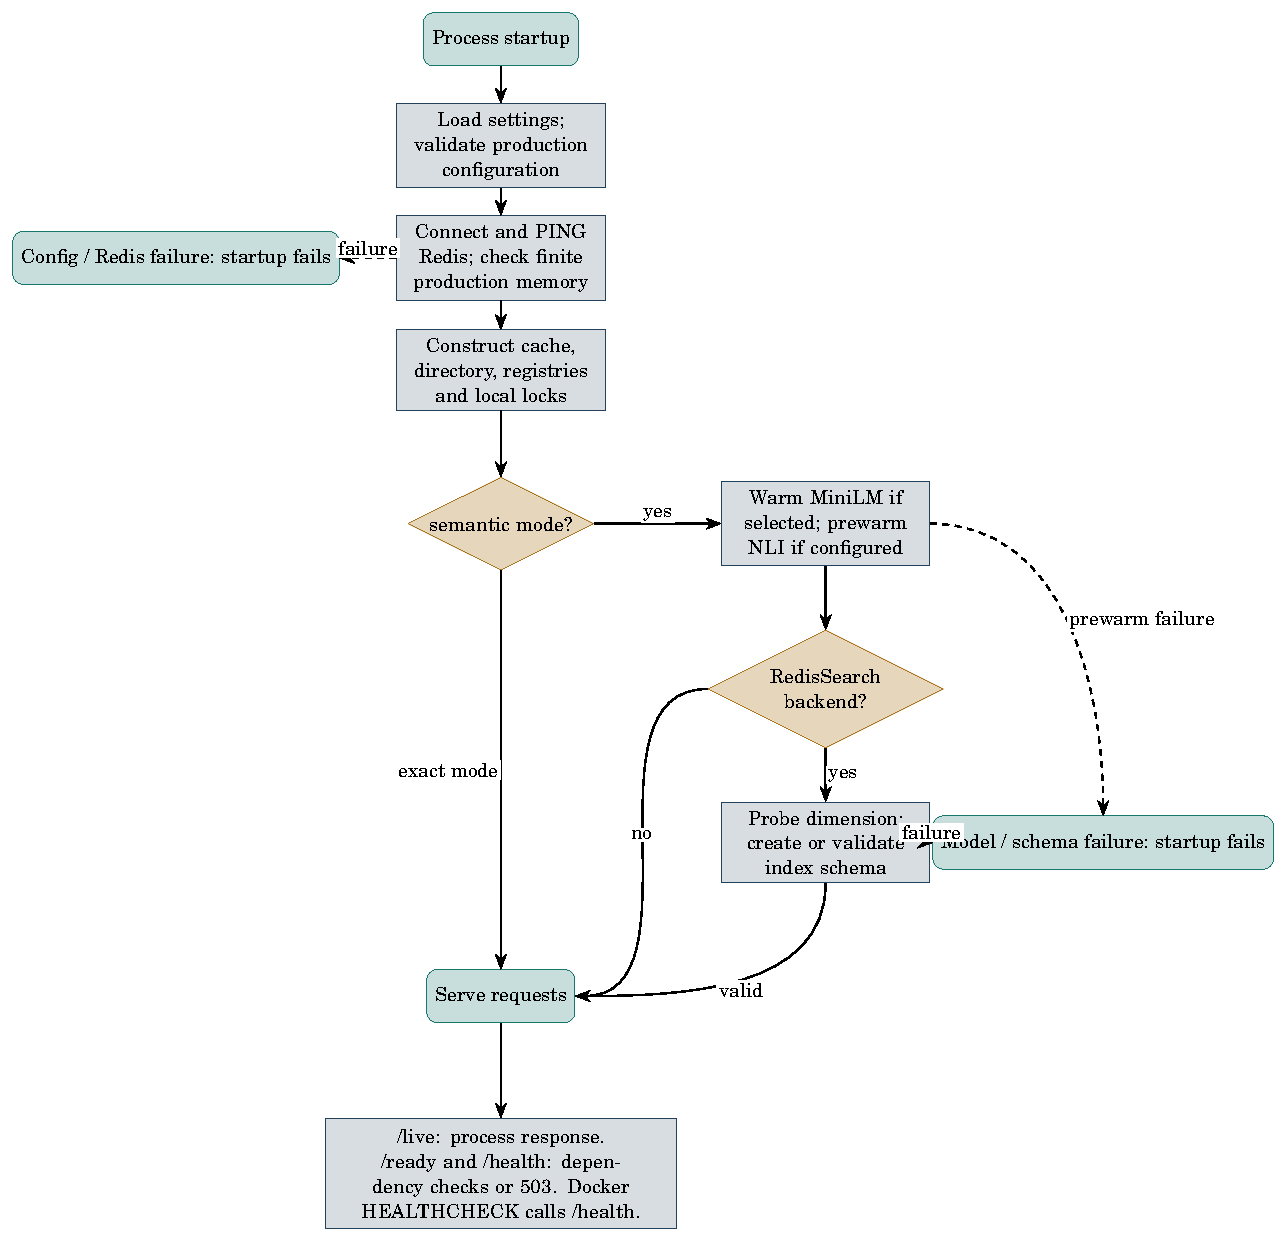
\includegraphics[width=\textwidth]{startup_readiness.pdf}
\caption{Conditional startup work and the implemented probe routes.}\label{fig:startup_full}
\end{figure}

\clearpage\thispagestyle{plain}
Figure~\ref{fig:lifecycle_full} separates processing from entry state. A completed response may be ineligible, explicitly no-store, a provider fallback, or a failed insertion; the generated answer can still be returned. A successful insert creates a hash and accounting metadata with a finite TTL. From the STORED state, lookup can update recency, TTL can expire the hash without a lookup, quota pressure can evict it by LRU, an authorized clear can remove it, or a same-key write can replace it. These transitions differ operationally: a touched entry may still expire, and a replacement begins a new residence period. A final candidate re-read catches a hash changed or removed while assessment was in progress.

\begin{figure}[H]\centering
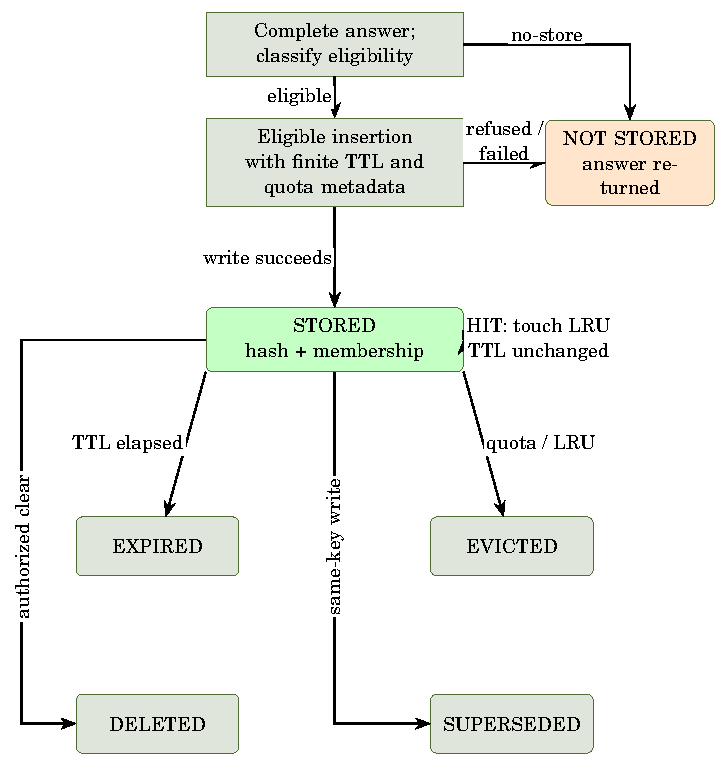
\includegraphics[width=\textwidth,height=.79\textheight,keepaspectratio]{cache_lifecycle.pdf}
\caption{Entry residence, recency touch, expiry, eviction, and deletion.}\label{fig:lifecycle_full}
\end{figure}
\clearpage

Consider one completed technical answer stored at noon with a finite TTL. A HIT shortly afterward moves its entry to the recent end of the scope and organization LRU order, but its hash keeps the original expiry. If that TTL elapses, Redis can remove the hash even without another request; a later vector result must be validated against the missing hash and cannot revive it. If the scope fills before expiry, an insertion can evict the least recently used live entry instead. These are distinct removal mechanisms and neither checks whether the technical advice remains factually current.

A same-key completed write replaces the answer and starts a new stored generation. A shortlist produced before that replacement is not permission to serve the old answer: the final read compares the chosen question and answer with the indexed candidate. An authorized private-cache clear similarly changes membership before a later lookup. The user-facing response can still be a provider MISS if a write was refused or failed, with storage metadata explaining why the generated answer was not retained.
